\documentclass{article}
\usepackage[english]{babel}
\usepackage[utf8]{inputenc}
\usepackage[T1]{fontenc}
\usepackage[hidelinks]{hyperref}
\usepackage{pgfplots}
\pgfplotsset{width=7cm,compat=1.18}
\usepackage{float}
\usepackage{subcaption}
\usepackage{booktabs}
\usepackage{amsmath}
\usepackage{array}
\usepackage{amssymb}
\usepackage{systeme}
\usepackage{tikz}
\usepackage{verbatim}
\usepackage{listings}
\usepackage{lipsum}

\begin{document}

\pagenumbering{gobble}

\begin{titlepage}
    \begin{figure}[!htb]
        \centering
        
\includegraphics[keepaspectratio=true,scale=0.5]{cherubinFrontespizio.eps}
    \end{figure}
    
    \begin{center}
        \LARGE{UNIVERSITÀ DI PISA}
        \vspace{5mm}
        \\ \large{DEPARTMENT OF COMPUTER ENGINEERING}
    \end{center}
    
    \vspace{15mm}
    \begin{center}
        {\LARGE{\bf Edge Computing\\Project Documentation}}
    \end{center}
    \begin{center}
        {
        \makeatletter    
        \@date
        \makeatother    
        }
    \end{center}
    \vspace{30mm}
    
    \begin{minipage}[t]{0.47\textwidth}
        {\large{Team:}{\normalsize\vspace{3mm} \bf\\ \large{Cavedoni F.\\Monaci M.\\Pinna F.}}}
    \end{minipage}
    
    \vspace{15mm}
    \hrulefill
    \\\centering{\large{ACADEMIC YEAR 2024/2025}}
\end{titlepage}

\newpage
\tableofcontents
\newpage

\pagenumbering{arabic}
\setcounter{page}{1}

\section{Introduction}
A cellular network is composed of M base stations, placed within a 2D floorplan of size L $\times$ H
according to a regular grid. Each base station also has edge computing capabilities, i.e., it can receive
computing tasks from cellular network's users and serve them at a rate equal to S instructions per
seconds following a First Come First Served (FCFS) policy. Assume that all base stations are
interconnected between each other via mesh topology.
\subsection{Problem description}
We consider N users placed at random locations \texttt{(x, y)} within the same 2D floorplan, where coordinates
\texttt{x} and \texttt{y} are random variables to be defined later. Each user generates a new computing task request
every T seconds, and each request consists of I instructions to be executed. T and I are exponentially
distributed RVs. In particular, a user sends each new task request to its serving base station (i.e., the
closest one), which in turn can follow one of methods below:
\begin{itemize}
    \item [\textbf{a)}] serve the request locally
    \item [\textbf{b)}] forward the request to the less-loaded base station
\end{itemize}

\subsection{Objectives}
This project aims to fulfill the following:
\begin{itemize}
    \item Evaluate the time required to complete a computing task for various values of N comparing method a) against method b)
    \item Evaluate the following scenarios:
    
    \texttt{x} and \texttt{y} are \textit{uniform distributed} random variables in range \[x\in[0, width] \quad y\in[0, height]\]

    \texttt{x} and \texttt{y} are distributed as a \textit{lognormal distribution} with parameters defined in \autoref{factors}
    \item \texttt{TODO\dots}
\end{itemize}

\subsection{Performance indexes}
\begin{itemize}
    \item Response time of the system (when a packet leaves the system)
    \item Response time of each queue
    \item Packet loss
    \item \texttt{TODO\dots}
\end{itemize}

\section{Modeling}
Our system is described by the following scheme
\begin{figure}[H]
    \centering
    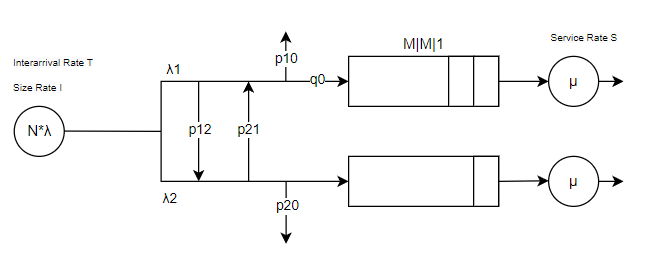
\includegraphics[width=\textwidth]{immagine.png}
    \caption{Scheme}
    \label{scheme}
\end{figure}

As shown in \autoref{scheme}, each base station is modeled as an \texttt{M/M/1/k} system, as rates $\lambda_i$ and $\mu_i$ are exponentially distributed random variables $\forall \ i \in [1, M]$.

\subsection{Assumptions}
We make some assumption in order to simplify the implementation of the system.

\begin{enumerate}
    \item Rerouting propagation delay is constant for each base station.
    \item Every job entering a queue is destined to be served and cannot exit the queue in any other way.
    \item Each queue length is \textit{finite} with \texttt{k} slots.
    \item \textit{(work in progress)} Width and height of the grid are such that it results in a square area.
\end{enumerate}

\subsection{Factors description}\label{factors}
\begin{itemize}
    \item \texttt{N}: number of users
    \item \texttt{k}: length of each queue
    \item $\lambda_i$: Interarrival rate for base station $i$
    \item $\mu$: Service rate for each base station
    \item $\mu_{log}$: Average of lognormal distribution
    \item $\sigma_{log}$: Standard deviation of lognormal distribution
\end{itemize}

\section{Implementation}
\subsection{Modules}
The following modules have been defined:
\begin{itemize}
    \item \textbf{EdgeNetwork}: compound module which represents the system and hosts the following simple modules
    \begin{itemize}
        \item \textbf{BaseStation}: simple module which receives, precesses and (in case of scenario b) forwards packets sent by users according to the specified distribution. 
        \item \textbf{User}: simple module which generates and sends packets (with length dependent by the specified distribution) to the nearest base station.
    \end{itemize}    
\end{itemize}

\subsection{Modules' behaviour}
\subsubsection{EdgeComputingNetwork}
\begin{itemize}
    \item Hosts base stations and users physically and memorizes their parameters in order to retreive them during the simulation via parent pointers.
\end{itemize}
\subsubsection{BaseStation}
\begin{itemize}
    \item Receives packets from users in form of \texttt{cMessage} objects and depending on the current scenario performs one of the following actions:
    \begin{itemize}
        \item [\textbf{Locally managed:}] if the queue has enough free slots the base station enqueues the packet to be processed, ignoring all other base stations.
        \item [\textbf{Forwarding:}] when a packet is received the base station searches for the base statio with the lowest load on their queue and forwards the packet to it. If and only if every other base station has a higher load, the packet is served locally.
    \end{itemize}
    \item It also records statistics every time a packet is \textit{dropped} or \textit{forwarded} (as number of packets) and about \textit{queue length} and \textit{response time} (in order to compute its average).
\end{itemize}

\subsubsection{User}
\begin{itemize}
    \item Generates packets with length and rate which are exponentially distributed and sends them to the \textit{nearest}\footnote{According to the euclidean distance}
    % non so se è superfluo specificarlo
    \texttt{BaseStation}.
\end{itemize}

\newpage
\section{Verification}
Right away we describe the tests made to verify if our system tends to remain stable under extreme conditions.

\section{Calibration}
We now talk about how factors and other parameters have been chosen throughout the developement.

\end{document}